%=========================================
% 	   Fallbeispiel     		 =
%=========================================
\chapter{Fallbeispiel}
In diesem Kapitel stellen wir, eine anhand eines selbst ausgedachten Anwendungsfalls, Cloud-Native Architektur vor, die wir prototypisch implementiert haben.

\section{Beschreibung}
Im Rahmen des Beispiels, haben wir eine Cloud-Native Architekturn für ein Chatprogramm (ChatApp) entworfen. Die Applikation soll drei Funktionen besitzen. Benutzer sollen sich registrieren können, Benutzer sollen sich ein-und ausloggen können und Benutzer sollen Nachrichten an andere Benutzer schreiben können. Im folgenden sind alle funktionalen und nichtfunktionalen Anforderungen aufgeführt.


\section{Anforderungen}
\subsection{Nichtfunktionale Anforderungen}
1. Skalierbarkeit
Das System muss mit einer großen Zahl von Benutzern, die das System gleichzeit verwenden, umgehen können.

2. Verfügbarkeit
Das System muss zu jeder Zeit verfügbar sein.

3. Sicherheit
Das System muss Berechtigungen überprüfen können (z.B. darf Benutzer X die Nachrichten lesen) und das System sollte sich gegen übliche Cyberangriffe (z.B. DDoS) schützen können.

4. Änderbarkeit/Erweiterbarkeit
Das System muss es zulassen, dass weitere Komponenten (z.B. Hochladen von Bildern und Videos) einfach hinzugefügt werden können.

\subsection{Funktionale Anforderungen}
1. Registierung
Ein Benutzer kann sich mit seiner E-Mail Adresse und einem Passwort im System registieren.

2. Ein- und Ausloggen
Ein Benutzer kann sich mit seiner E-Mail Adresse und seinem Passwort im System anmelden und danach die Funkionen nutzen bis er sich abmeldet.

3. Nachrichten schreiben/lesen
Ein Benutzer kann Nachrichten an andere Benutzer senden und Nachrichten, die an ihn gesendet worden sind, abrufen.


Im nächsten Abschnitt stellen wir die von uns entworfene Architektur vor und erläutern die wichtigsten Merkmale. 

\begin{figure}[bth] 
	\centering
	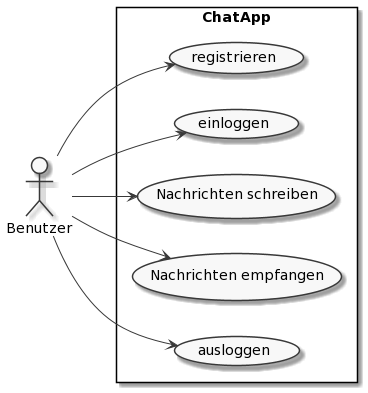
\includegraphics[width=0.6\textwidth]{Graphics/Usecase-Diagramm.png}
	\caption{Use-Case Diagramm}
\end{figure}

\section{Architekturentwurf}

\section{Übersicht}
Wie in Abbildung xx zu sehen ist besteht die Architektur aus einem Client mit graphischer Oberfläche (UI) einem API-Gateway, das alle Anfragen von Clienten empfängt und drei Microservices mit je einer eigenen Datenbank, die die Hautpfunktionalitäten des Systems implementieren.

\subsection{Microservices}
Jede Funktion aus den Anforderungen korrespondiert mit einem Microservice. Die Aufteilung der Microservices ergibt sich aus der Annahme, dass die Funkionalitäten, die sie bereitstellen unterschiedlich oft genutzt werden: Anzahl der Registrierungen < Anzahl Login/Logout < Anzahl der geschriebenen Nachrichten/Abruf von Nachrichten). Dadurch kann jede Funktion/Microservice individuell hoch- oder runterskaliert werden ohne unnütze Resourcen zu verschwenden.

verfügbarkeit
ändrebarkeit
jeder service eigene datenbank

kommunikation

\subsection{API-Gateway}
Das API-Gateway schottet die Microservices ab. Die Abschottung hat mehrere Vorteile. Sicherheitsrelevante Aspekte wie z.B. DDOS-Protection oder der Schutz vor unbefugtem Zugriff (von Adressen, die nicht zum Client gehören) können auf das API-Gateway verlagert werden und müssen daher nicht in jedem Microservice implementiert werden.
Des Weiteren erfüllt das API-Gateway die Rolle eines Load-Balancers, sodass eingehende Anfragen auf Microservices verteilt werden können.

\subsection{Client}
Mithilfe des Clients können Anfragen an das System, genauer gesagt das API-Gateway, gesendet werden. Er enthält keine Funktionalitäten und dient lediglich zum Abrufen und Darstellen von Inhalten.


\begin{figure}[bth] 
	\centering
	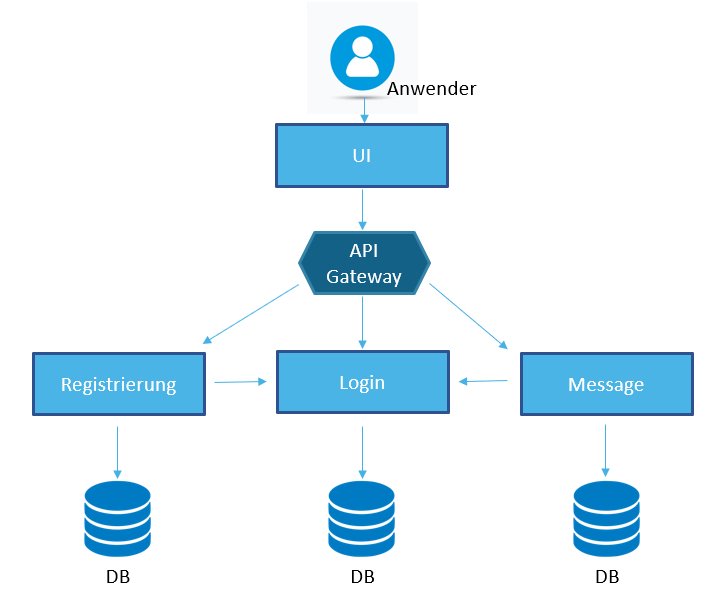
\includegraphics[width=0.6\textwidth]{Graphics/Architekturentwurf.png}
	\caption{Architekturentwurf}
\end{figure}

\begin{figure}[bth] 
	\centering
	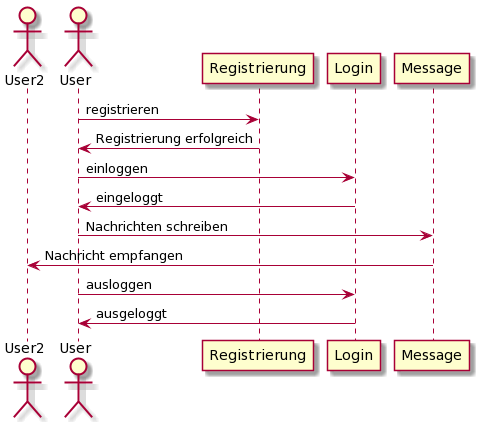
\includegraphics[width=0.6\textwidth]{Graphics/Sequenzdiagramm.png}
	\caption{Sequenzdiagramm}
\end{figure}

\section{Implementierung des Prototyps}
java
react
http
datenbank
stove pipe
einzelne programme die individuell gestartet werden können

auch genutzte Technologien aufzeigen

